\chapter{The Architecture of the SAFE Network}
\label{ch:architecture}

The internet is constantly growing and changing. Changes in technologies slowly permeate throughout the network as if by osmosis. Governmental policy can have a large impact on how people interact with the network, whether that be Turkey blocking Wikipedia or the US abandoning Net Neutrality. This area is where the SAFE Network starts to deviate greatly from the \textit{traditional} internet. The SAFE Network is a 'Autonomous Data Network'. To have access to the SAFE Network means to have access to all of it. A government cannot curate access data. This is made possible by the architecture of the SAFE Network.

\section{Vaults and Clients}

The SAFE Network is comprised of \textit{vaults}. A \textit{Vault} is a singular program/application that a user runs on their computer, whether that be a server hosted in a datacenter, a Raspberry Pi or a desktop computer. A \textit{vault} is given a set amount of storage by the user which it then uses to \textit{farm} data. For a given \textit{vault} to join the network, it must pass a 'Proof of Resource'. This initial test is used to validate that the \textit{vault} has enough bandwidth and CPU power to be able to adequately perform its job. Similar to how a real world farmer looks after their crop/animals, a \textit{farmer} (\textit{vault}) on the SAFE Network looks after data. Understanding that nomenclature is quite useful in understanding the function a \textit{farmer} (\textit{vault}) serves. Once \textit{vault} is successfully storing data it is rewarded with \textit{Safecoin}, which is a cryptocurrency hosted on the SAFE Network. Reading data from the network doesn't incur any cost, it is only when writing data that a user (\textit{client}) has to expend \textit{Safecoin}. A user doesn't need to run their own \textit{vault} to interact with the network, all users interact through the use of a \textit{client}. To help increase privacy, a \textit{client} connects to the network through an intermediary \textit{vault} called a \textit{proxy node}. This \textit{proxy node} orchestrates the writing and retrieval of data on behalf of the \textit{client}, hiding the \textit{clients} IP address from the rest of the network.

The only time a user interacts with their \textit{vault} is through configuration before startup. The most notable configuration being the allocation of storage for the \textit{vault}. Once \textit{vaults} start communicating with each other there is no intervention by humans. The network itself votes on and decides many factors. This includes everything from where data should be stored to how much value a \textit{Safecoin} has. This is the autonomy of the network, it does not accept governance by humans and \textit{vaults} cooperate for the good of the entire network.

\subsection{Self-Encryption}

Data that is stored on the SAFE Network is split up into small 1MiB chunks through a process called \textit{self-encryption}. Each 1MiB chunk of data is then hashed to give a unique address in 256-Bit XOR Address Space.

\subsection{Disjoint Sections}

The unique address of every 1MiB chunk from \textit{self encryption} is used to determine what \textit{vaults} are responsible for storing it. Maidsafe's innovation was in the creation of what are called \textit{Disjoint Sections}. These \textit{sections} are groups of vaults that are responsible for a certain range of the 256-Bit XOR Address Space. By default, the network requires a minimum number of vaults to sustain the network. At the time of writing this is 8 vaults. These 8 vaults form a complete 'section' and are responsible for the storage of the entire 256-Bit address range. As more vaults join the network, this \textit{section} will grow in size and then eventually split into two new \textit{sections}. There are numerous requirements that have to be met before a \textit{section split} is allowed.

% Insert equation for section split

After a split, \textit{sections} are then responsible for half of the 256-Bit address range that they were before. As more and more complete \textit{groups} of ~8 \textit{vaults} join the network, it continues to split and each \textit{section} is therefore responsible for the curation of less and less data. An important thing to note is that the SAFE Network doesn't assign 256-Bit addresses based on proximity, in a given section two \textit{vaults} could be very close together in 256-Bit XOR space but be located on different continents. This property helps the integrity of the network by ensuring \textit{vaults} in a given section are not located close to each other. Otherwise the network could be open to simple attacks. For example, start 8 \textit{vaults} on a single computer to form a \textit{section} then suddenly switch them all off which could cause data loss. If a significant number of \textit{vaults} leave the network then \textit{sections} have the ability to join with other \textit{sections} to ensure the stability of data is maintained. In Figure \ref{fig:safe-sections} you can see four \textit{sections} comprised of four \textit{vaults} each, you can see the address range that each \textit{section} is responsible for. In the diagram four \textit{vaults} make a \textit{section} instead of the traditional eight, this is just to make the diagram easier to process.

\begin{figure}
	\begin{center}
		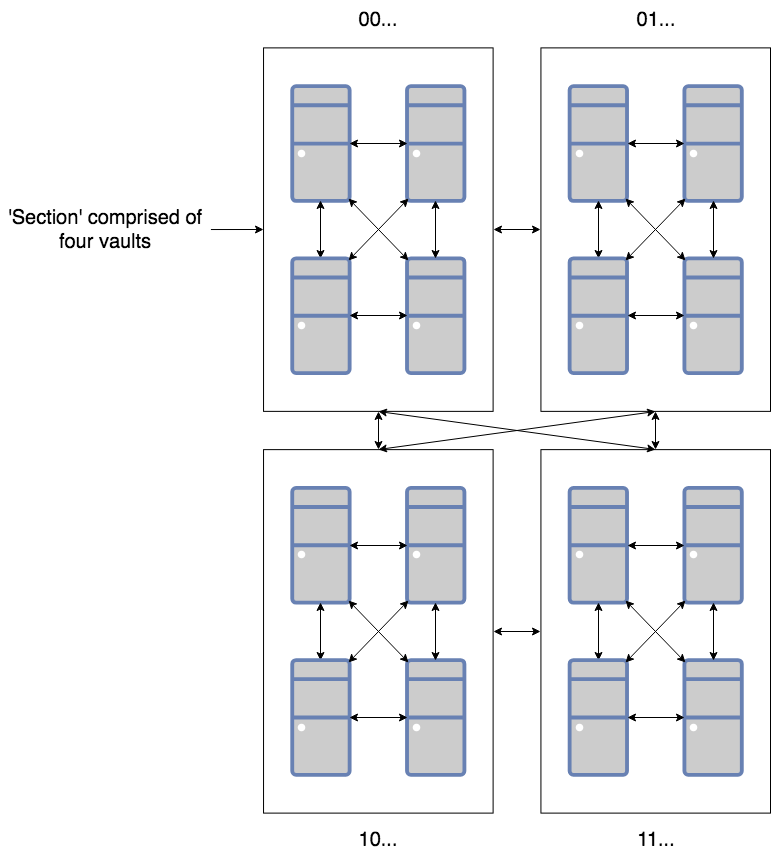
\includegraphics[scale=0.3]{diagrams/safe-network-sections}
		\caption{Four sections of a SAFE Network. You can see the address range each section is responsible for.}
		\label{fig:safe-sections}
	\end{center}
\end{figure}

\subsection{Proof of Resource}

The \textit{proof of resource} (PoR) test is used to valid the effectiveness of a \textit{vaults} ability to store and serve data and is the value proposition of \textit{Safecoin}. The PoR is used to validate \textit{vaults} joining the network but also during other network events. The process is as follows:

\begin{itemize}
	\item 
\end{itemize}

\subsection{Personas}

Vaults can be characterised as having different 'Personas'. The most \textit{basic} persona that a vault can have is that of the Data Manager. A Data Manager is responsible for the storage of chunks within a section. Their job is vital to the stability of the network. When data is stored on the network, it is actually 'duplicated' across multiple Data Managers. At all times the network aims to keep a minimum number of copies of a chunk of data, if a chunk goes missing (say a vault goes offline) this chunk is quickly duplicated to another Data Manager to ensure that data is stored redundantly. Hence within a given section, there will be several vaults storing identical chunks of data. Each having full knowledge of the chunks of data that the other Data Managers hold. The other persona a vault can take is that of the Client Manager. A Client Manager is responsible for storing the account data for clients. When you create an account on the SAFE Network, that data is stored like any other piece of data on the network. It has a given 256-Bit Address and contains the information like: how much Safecoin an account has, the number of chunks of data that has been uploaded, etc. As an account is a 256-Bit address it will fall within the domain of a particular section, the Client Managers in that section will then store the relevant data. As I will discuss in the section on Encryption, a vault does not know the IP address of the client that it is interacting with. The Client Manager thus doesn't know the IP address of the client it belongs to, it is just data and they cannot arbitrarily read the account data because it is encrypted.

\subsection{Accounts}

\section{Crust and Encryption}

Crust is the secure routing layer used by the SAFE Network. It was designed and built by Maidsafe to provide the secure communications backbone of the SAFE Network. Crust allows for reliable peer to peer connections and provides encryption for all traffic. I won't go into too much detail but some important points to realise is that Crust doesn't have a standard port required to function, it is capable of randomising ports. Several Transmission Protocols can be used, falling back to UDP from TCP (for example) if required. Encryption at this level means that Data on the network is always encrypted, data is only decrypted client side and whenever it is not on a clients computer it is fully encrypted.

Encryption is a very important aspect of the SAFE Network. Whenever data is stored on the network, it is encrypted. As mentioned above the only time data is unencrypted is when it is on a client. Data on the network exists as discrete 1Mb chunks, each with its own 256-Bit Address. When a file is uploaded to the network, it undergoes a process known as self-encryption. Self-Encryption is a pioneering technique developed by Maidsafe and is used to encrypt data. What happens is that when your file is broken down into 1Mb chunks, each chunk is encrypted with the hash of one of the other chunks. What happens then is a DataMap is constructed, this DataMap then contains the addresses of each of these individual chunks of data so that they can be retrieved. As data is stored on the network in this manner, you have a number of options on how to access it. You can choose to have data "unencrypted" or what Maidsafe calls "Plain", what this means is that any user that knows the address of the data (and the type-tag) can retrieve and read the data. The special thing about this is that the data is still fully encrypted on the network through self-encryption, a vault owner cannot decipher what the chunk of data holds. When anyone goes to access this data though, it is reassembled and you can read it. The two other types of encryption supported are Symmetric and Asymmetric. Having these options means that you can build applications in quite a flexible manner. A user can freely share the key to data and this opens up the possibility for interesting designs.

A system is also in place to protect a users identity as they connect to the network. This aspect of the SAFE Network is very important to my project. When a client connects to the network, they do so through the use of a \textit{Proxy Node}. A Proxy Node is a vault that is used to liaise between a client and the network at large. When a user connects, the Proxy Node of course knows the the IP address of that client. Beyond the Proxy and deeper into the network all the vaults know is the XOR Address of the account being used (including other relevant data and public encryption keys). Hence by using a Proxy Node, the activity of the client is well hidden from the rest of the network. A given vault cannot detect that the data being retrieved is going to someone in a particular country etc. This means that clients can anonymously read and store data to the network without people being able to monitor the contents of that data. I will touch upon this later on when I discuss my project, this anonymity is very important. In Figure \ref{fig:proxy-connection} you can see the topology of how a client connects to the SAFE Network.

\begin{figure}
	\begin{center}
		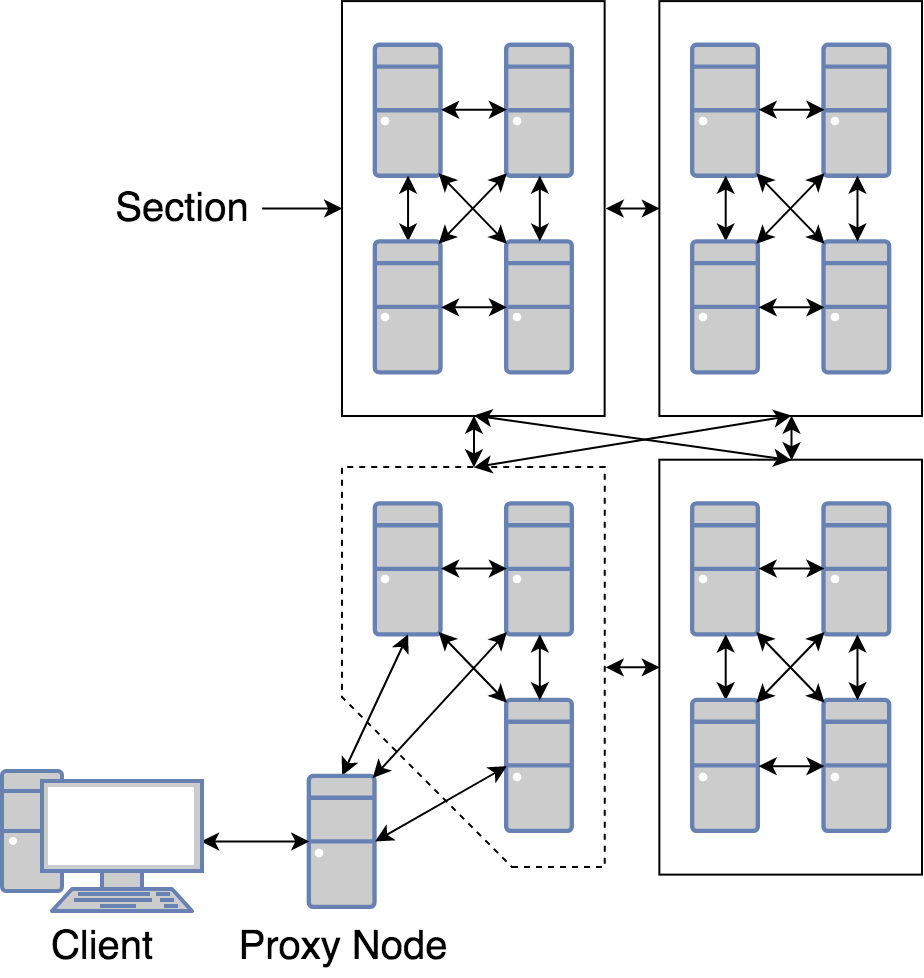
\includegraphics[scale=0.35]{diagrams/safe-network-connection}
		\caption{A client connecting to the SAFE Network through a Proxy Node}
		\label{fig:proxy-connection}
	\end{center}
\end{figure}

\section{Safecoin}

Safecoin is the cryptocurrency of the SAFE Network, it is earned by farmers and spent by writing data to the network. The expectation is that as the cost of CPU/Storage falls with time, the value of the Safecoin will increase. As in, the amount of raw bytes that a given Safecoin would allow the storage of increases.

\section{Quorum and the Datachain}

As the network acts as an autonomous entity, there has to be some method for a given vault to reach consensus with other vaults. This problem is what Cryptocurrencies aim to solve through processes such as mining. Mining is essentially the network reaching consensus upon what has happened (in this case, financial transactions). In the case of Bitcoin, every time a block is mined, it is cryptographically linked to the block that came before it. As this \textit{Blockchain} grows in size, the consensus on past transactions grows and grows. For Bitcoin and similar cryptocurrencies, to be able to undo a transaction/block you would need to have control of over \%50 of the networks hash power. The debate on how easy it is to do that is a hotly debated topic that is outside the scope of this paper. The SAFE Network needs a similar mechanism on how to reach consensus. Analogous to a Blockchain, the SAFE Network has a 'Datachain'. This Datachain is used to help insure the integrity of the network and can be used to help rebuild the network incase of a catastrophic failure. For any action on the network to be valid, whether this be the storing of data or a vault joining a section, there has to be a corresponding 'group signature'. This group signature is stored in the Datachain that all vaults in a section has. In order for an action to be valid, a section has to reach a 'quorum'. For a network where the minimum section size is eight, a quorum would be five out of the eight vaults. This means that in a given section, several vaults could be acting as 'bad parties' but network integrity wouldn't be lost. XOR Distance also comes into play in this process. The closer two sections are in 256-Bit XOR Address Space the more they know about the data the other section is storing. They will have access to the portion of the Datachain that is used by that section. This way, a given section can help to verify that a neighbour is acting as a good party in the network and that data being stored there has not been tampered with. The further away in 256-Bit Address Space two sections are then the less they know about each other. This means that as the number of sections increases, the influence a given a section has over the network decreases. Eventually resulting in no section in the network having an overview of the entire network.

A protection mechanism exists in the retrieving of data to account for the case when a vault tampers with data after it has been recored in the Datachain. When a client requests a given piece of data, a single vault is chosen to return that chunk of data corresponding to a 256-Bit address. Alongside the data that is returned, a minimum number of acknowledgements from other vaults in the section must be returned too. This way, a client can then verify the data they receive against the acknowledgements from the other vaults in order to ensure that the data is valid.

The development of the Datachain is still very active, at the time of writing I have tried my best to summarise the current proposals. Things are subject to change as Maidsafe runs simulations and exams how things operate.

\subsection{Node Age and Churn}

A crucial part of the integrity of the Datachain is node ageing. In order for a vault to \textit{vote} on network activity (this is the signatures that form the group signature) it has to have proved itself a reliable party. A vault cannot just join the network and start voting in network decisions. When a new vault announces itself to the network, it is issued with the Proof of Resource that we discussed earlier. If it passes the proof of resource then as long as the assigned section reaches a quorum on the new vault joining, then it joins that section. This node is very 'young' in the eyes of the network and as such is not trusted. It is not allowed to vote in group actions and is responsible only for the storage and transmit of data. A very interesting aspect of the SAFE Network is the concept of \textit{churn}. Churn is used to constantly 'rotate' vaults round different sections on the network. This means that in a given time frame, a vault will not be responsible for the same 256-Bit address range. This important feature helps to ensure that it is very difficult to track down where data is stored in order to erase it or corrupt it. During churn, young vaults with a lower node age will be chosen more frequently than older vaults. The vault is assigned to a new section, to which it must give another proof of resource. If the new section reaches quorum then the vault joins that new section and its node age is incremented. Thus, trust must be earned by acting as a good party in the network over time. Only when a node reaches a certain node age does it become an \textit{elder}. An elder is a node which has a high node age, meaning it has been up and running for a while and has proven itself to be a reliable party. When a node is an elder, it gains the voting writes that eventually lead to the construction and maintenance of the Datachain. Vaults that are not elders have no voting writes and essentially just do what they are told by the elders. If a vault acts out of order then its node age can be decremented or eliminated entirely. Trust must be earned.

Node ageing and churn are hence essential security features of the network and make it very difficult for an attacker to have any choice in the section of the network they wish to attack.

\section{Immutable and Mutable Data}

Data stored on the SAFE Network can take one of two forms. It can either be \textit{Immutable Data} or \textit{Mutable Data}. A Mutable Data Structure (often abbreviated MD) is a key value storage mechanism that allows for the storage of 1000 entries at a maximum size of 1Mb. A MD has a 256-Bit address to specify its location. An Immutable Data Structure only stores a single 'value', its address on the network is derived from the hash of binary data it contains. An Immutable Data structure can itself only be 1Mb in size, but through the use of a Data-Map this limit can be subverted. I will talk more in depth about the Data-Map when we discuss my project, as its properties are very important to my application. As their names imply, Mutable Data can be freely changed and updated whereas Immutable Data cannot. Its clear to see that if you change the contents of Immutable Data then it will no longer correspond to the address at which it is stored. As mentioned previously, it is this property of Immutable Data that eliminates duplication on the network. If a user uploads the same file as another user they are simply presented with another \textit{key} to access that data. If a user 'deletes' the data it will remain on the network as another user still maintains the key to access it.

\section{Privacy and Anonymity}